


\section{Formação de mamteriais cristalinos}
Materiais alotrópicos ou polimórficos apresentam mais de uma estrutura cristalina.

\textbf{Alotropia}: substâncias puras.

\textbf{Polimorfismo}: Substancias compostas

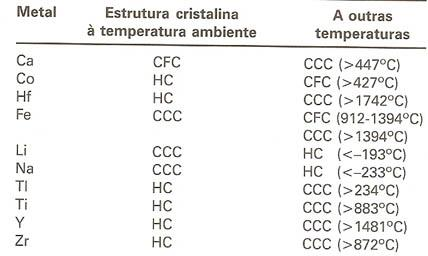
\includegraphics[scale=0.4,trim={0 0 0 0}]{figures/estruturaTemp}

O processo de formação de cristais pode ser através de processo natural, em laboratório ou na indústria.

O crescimento se dá sob forças acidentais, presença de íons estranhos, variação da temperatura.

Podem ainda ser feitor a partir:

\begin{itemize}
	\item Solução;
	\item Vapor;
	\item Massa em fusão.
\end{itemize}


Cada ponto de cristalização é chamado de núcleo de cristalização e a formação destes núcleos pode ser:

\begin{itemize}
	\item Homogênea: núcleos formados pelos átomos de próprio metal 
	\item Heterogênea: núcleos formados sobre um substrato ou outro material presente. Requer menor energia para formação de núcleo estável do que na própria substância.
\end{itemize}

A depender do número de núcleos presentes no material, este pode ser classificado como monocristalino e policristalino. As propriedades mecânicas podem variar de acordo com o número de núcleos cristalinos.

É observado experimentalmente que os materiais policristalinos apresentam defeitos, i.e. rachaduras e falhas, nas regiões entre os núcleos de cistalização.


\section{Soluções Sólidas}

Poucos metais são utilizados na sua forma pura. Sendo assim, grande parte dos materiais são chamados de ligas metálicas por haver combinação de dois ou mais metais.

Se o limite de solubilidade é ultrapassado, uma nova fase é formada e observada nesses materiais.

Exemplos de ligas metálicas:

\begin{itemize}
	\item Ligas de cobre: latão / bronze / cupro-níquel atãobronze
	\item Ligas de níquel: monel/ inconel/ incoloy
	\item Ligas ferrosas: Aço-C / Aços inoxidáveis
\end{itemize}

\section{Elementos de Liga}

Os elementos de liga são impurezas adicionadas intencionalmente e podem promover a melhora de algumas propriedades desses materiais e torná-lo útil para outras aplicações tecnológicas. Algumas características são:

\begin{itemize}
	\item dopagem em semicondutores;
	\item maior resistência mecânica;
	\item maior resistência a corrosão;
	\item maior condutividade elétrica;
	\item melhor soldabilidade.
\end{itemize}


\section{Soluções Sólidas}

Tipos de soluções sólidas:

\begin{itemize}
	\item substitucional: o átomo do elemento acrescido a liga substitui a posição de um dos átomos presentes na célula cristalina;
	\item intersticial: o átomo do elemento acrescido a liga invade o interstício dos átomos que formam a célula cristalina .
\end{itemize}


As soluções sólidas SUBSTITUCIONAIS podem ainda ocorrer de forma 

\begin{itemize}
	\item Ordenada;
	\item Ao acaso.
\end{itemize}

\section{Regras de Hume-Rothery}

\begin{itemize}
	\item Variação \% causada pela diferença entre raios < 15\% (evitar distorções na rede): raio soluto = raio solvente/
	\item Mesma estrutura cristalina;
	\item Eletronegatividades semelhantes
	\item Mesma valência.
\end{itemize}



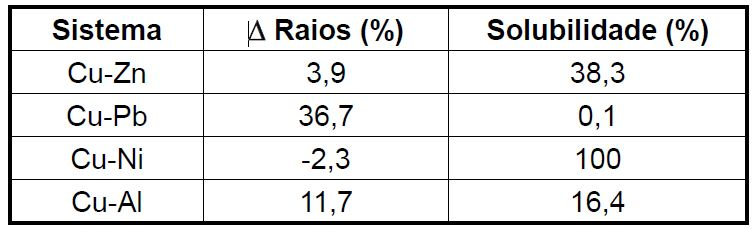
\includegraphics[scale=0.4,trim={0 0 0 0}]{figures/hume}


{\LARGE VER COMO É ESSA REGRA EM UM LIVRO DAS REF}

{\LARGE NECESSÁRIO TERMINAR ESSE TÓPICO COM FORMULAS}


\section{Imperfeições Cristalinas}

É uma imperfeição no arranjo periódico regular dos átomos em um cristal. Podem estar relacionada à posiçãodos átomos ou ao tipo de átomo presente na rede.

\textit{O tipo e o número de defeitos dependem do meio ambiente, do material e das circunstâncias sob as quais o cristal é processado.}

\begin{itemize}
	\item Representam pequena fração da rede mas podem significar muito nas propriedades dos materiais.
	\item Podem permitir a introdução de elementos de liga formando novos materiais.
\end{itemize}

Defeitos pontuais:

\begin{itemize}
	\item Lacunas ou vazios simples ou não.
	\item Originadas por perturbações locais durante a solidificação ou vibrações térmicas a altas temperaturas.
\end{itemize}

Defeitos em sólidos iônicos:

\begin{itemize}
	\item \textbf{Defeito de Schottky}: vazio de par de íons (exclusivo de materiais iônicos) AX $\rightarrow$par consistindo de lacuna de cátion e lacuna de ânion $\rightarrow$ neutralidade.
	\item \textbf{Defeito de Frenkel:} deslocamento de um íon para um interstício (muita energia adicional) $\rightarrow$lacuna de cátion + cátion intersticial $\rightarrow$Não existe alteração de cargaImperfeições
\end{itemize}


Contorno de grãos:

\begin{itemize}
	\item Formada entre cristais (contornos de grãos) ou nas superfícies externas.
	\item No contorno dos grãos, os átomos não estão à mesma distância uns dos outros. Há tensões de tração e compressão.
	\item Influenciam nas propriedades físicas (ex: resistência mecânica) e químicas.
	\item Ajuste do tamanho dos grãos $\rightarrow$ uma das formas de controle das propriedades de um metal.
	\begin{itemize}
		\item Ex: Reduzindo o tamanho dos grãos, há aumento do área de contorno de grão, diminuindo a distância percorrida pelas discordâncias aumento da resistência mecânica do material.
	\end{itemize}
\end{itemize}

Defeitos de linha:

São imperfeições lineares em cristais, que envolvem a aresta de um plano extra de átomos. Podem ser originados durante solidificação ou por deformação plástica.

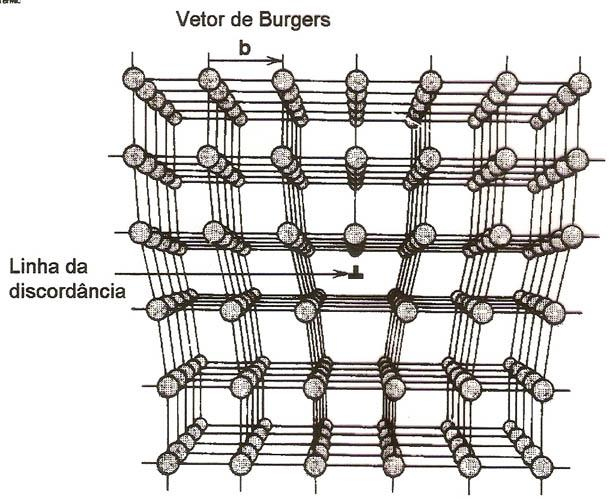
\includegraphics[scale=0.4,trim={0 0 0 0}]{figures/defLinhas}

\begin{itemize}
	\item Os defeitos (discordâncias, defeitos pontuais e contornos de grãos) atuam como barreiras para as discordâncias.
	\item O cisalhamento se dá mais facilmente nos planos de maior densidade atômica, que depende a orientação cristalográfica.
\end{itemize}


Fundamentos da Ciência e Eng. dos Materiais –uma abordagem integrada, Willian D. Callister, 2aed., Livros Técnicos e Científicos Editora, 2006.

Princípios de Ciência e Engenharia de Materiais. William F. Smith, 3ª ed, Editora Mc Graw Hill, 1998.

Ciência e Engenharia de Materiais: uma introdução, Willian D. Callister, 5a ed., Livros Técnicos e Científicos Editora, 2002.

